% Chapter 1

\chapter{Introduction}
\label{Chapter1} 

A distinctive trend of the twenty-first century is the slow but steady increase of the average age of the world population, that in the next decades will impact several aspects of our lives. Indeed, according to a US research \cite{ruder2008challenges}, people aged over 65 will increase by 101\% between 2000 and 2030. As a consequence, there will be an increment of the difficulty in taking care of elderly or vulnerable people within their own family.
For this reason, many companies and research teams are developing care-based technological solutions. 
The BRIDGe (Behavior dRift compensation for autonomous and InDependent livinG) project, developed by the research team of ATG (Assistive Technology Group \cite{b119}) of Politecnico di Milano, as we will see detail in section \ref{BRIDGeDescription}, is a very promising one.

Within this chapter we are going to introduce the reader to the problem context, discussing the works motivations, the goals and picturing a panoramic about the BRIDGe project.

\dots

\section{BRIDGe Project}
\label{BRIDGeDescription}
Behavior dRift compensation for autonomous and InDependent livinG (BRIDGe) is a complex system under development at the ATG of Politecnico di Milano. 

\dots

\subsection{BRIDGe Architecture}
Two main subsystems, one local and one remote, compose the BRIDGe system. The local subsystem, installed inside the environment, is characterized by low power computation and low voltage components such the home automation devices, sensors and a local small server (such as Raspberry PI).
The remote subsystem, located within the university labs, is based on more powerful hardware for analysis over a long period of time. This analysis is useful to understand the habits of the person as the time passes and their evolution. \ref{fig1.1}
\begin{figure}[ht!]
\centering
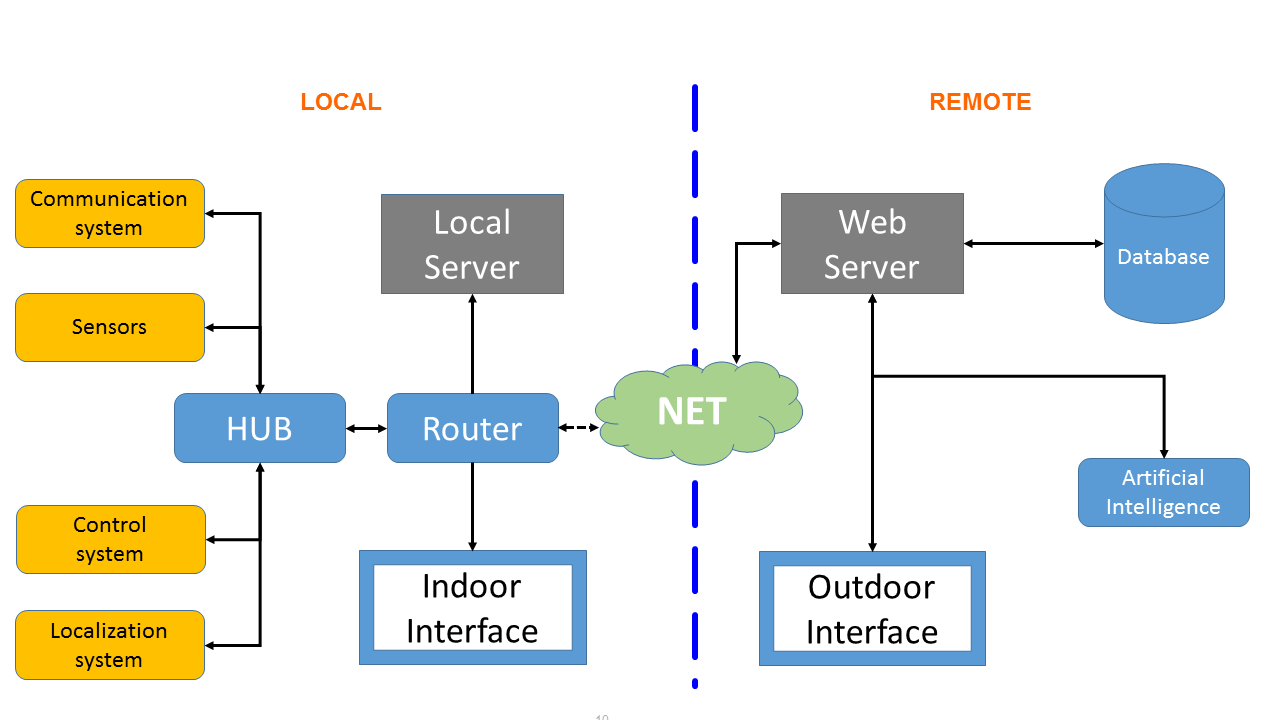
\includegraphics[width=140mm]{figures/ch1/fig7.png}
\caption{BRIDGe Architecture \label{overflow}}
\label{fig1.1}
\end{figure}